\section{new section}\label{new-section}

\begin{itemize}
\itemsep1pt\parskip0pt\parsep0pt
\item
  item

  \begin{itemize}
  \itemsep1pt\parskip0pt\parsep0pt
  \item
    item 1.1
  \item
    item 1.2
  \item
    new item
  \end{itemize}
\end{itemize}

\[
\begin{aligned}
x_i &= y_i \\
x_i + y_i &= y_i
\end{aligned}
\]

cite me: \textcite{Abb97}

\begin{Shaded}
\begin{Highlighting}[]
\NormalTok{x <-}\StringTok{ }\DecValTok{1}
\end{Highlighting}
\end{Shaded}

\begin{Shaded}
\begin{Highlighting}[]
\KeywordTok{plot}\NormalTok{(}\DecValTok{1}\NormalTok{:}\DecValTok{10}\NormalTok{)}
\end{Highlighting}
\end{Shaded}

\begin{figure}[htbp]
\centering
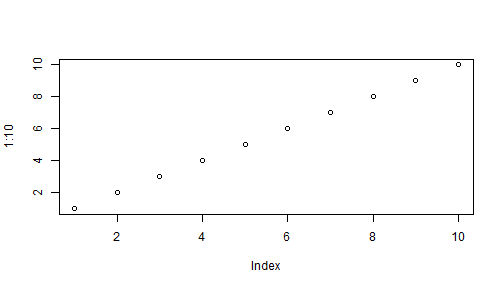
\includegraphics{figs/test/unnamed-chunk-2-1.png}
\caption{plot of chunk unnamed-chunk-2}
\end{figure}
